\section{Theorie}
\label{sec:Theorie}
Mittels der Kernspinresonanz
können ein Teile der magnetische Momente von Atomkernen
in einer Probe
durch Anlegen eines
äußern Magnetfeldes
gezielt verändet werden und somit
eine makroskopische Magnetisierung der Probe
erzeugen.
Durch die Kernspinresonaz ist es möglich
Aussagen zur Molekulstruktur wie z.B. chemischen Bindungen
zu machen.
Desweiteren können auch mikroskopische
Relaxationsprozesse innerhalb der Probe
durch anlegen eines
äußern magnetischen Wechselfeldes
untersucht
werden.


% Einleitung
% kurze zusammen fassung kernspinresonaz
\subsection{Kernspinresonaz}
Zunächst soll die Magnetisierung einer Probe
in einem Magnetfeld $\vec{B}=B_0\vec{e}_z$,
die sich im thermischen Gleichgewicht befindet, betrachtet werden.
Durch den Zeeman-Effekt
spalten sich die Kernpinzustände mit
Spinquantenzahl $I$ in
 $2I+1$ äquidistante Unterniveaus auf.
 Die Unterniveaus werden mittels
 der Orientierungsquantenzahl $m$
$(-I \leq m \leq I)$ unterschieden und
benachbarte Niveaus besitzen die Energiedifferenz
\begin{align*}
  \Delta E =\gamma B_0 \hbar.
\end{align*}
Die Besetzung im thermischen Gleichgewicht
bei der Temperatur $T$ erfolgt nach der
Bolzmann-Verteilung. Es folgt demnach
für das Besetzungsverhältnis zweier benachbarter Niveaus
\begin{align}
  \frac{N(m)}{N(m-1)} &= \exp\left(-\frac{\gamma B_0 \hbar }{k_B T}\right).
\intertext{Durch die ungeleiche Besetzung
ergibt sich eine Kernspinpolarisation}
\langle I_z \rangle &= \frac{\sum_{m=-I}^{m=I}\hbar m \exp\left(-\frac{m\gamma B_0 \hbar}{k_B T} \right) }{\sum_{m=-I}^{m=I}\exp\left(-\frac{m\gamma B_0 \hbar}{k_B T}\right)}. \label{eqn:I_z}
\end{align}

Werden nur Protonen betrachtet, ergibt
sich, da $I=\tfrac{1}{2}$
eine Aufspaltung, die in der
Abbildung \ref{fig:Proton} dargestellt ist.

\begin{figure}
 \centering
 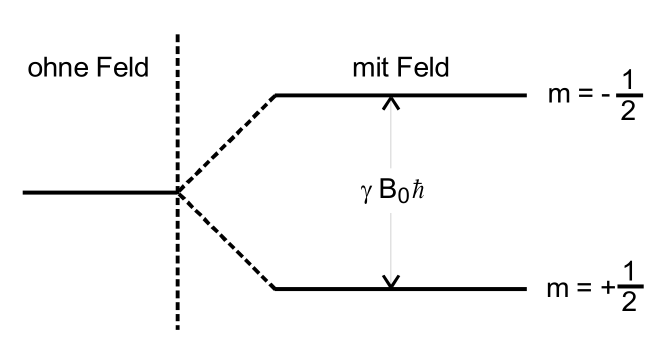
\includegraphics[width=0.5\textwidth]{Zeeman.PNG}
 \caption{Aufspaltung der Energieniveaus im Magnetfeld $B_0$ für $I=\tfrac{1}{2}$.}
 \label{fig:Proton}
\end{figure}
Für Zimmertemperatur und Magnetfelder
der größenordnung $\SI{1}{\tesla}$
gilt $m\gamma B_0 \hbar \ll k_BT$.
Die Kernspinpolarisation für Proton
vereinfacht sich
durch die Näherung zu
\begin{align}
\langle I_z\rangle_P= -\frac{\hbar^2}{4}\frac{\gamma B_0}{k_B T}.
\end{align}
Für die Gleichgewichtsmagnetisierung $M_0$ bei der
der Temperatur $T$ in $\vec{e}_z$-Richtung gilt dann
\begin{align}
M_0=\frac{1}{4}\mu_0 \gamma^2 \frac{\hbar^2}{k_B} N \frac{B_0}{T}
\end{align}
mit $N$ der Anzahl der Momente pro Volumeneinheit.

\subsection{Larmor-Präzession??}
\label{subsec:zielsetzung}
Durch die große Anzahl von Einzelmomenten in einer Probe \approx $\SI{10e28}{\per\cubic\meter}$
kann die Probenmagnetisierung $\vec{M}$ mit klassischen Methoden
beschrieben werden.
Auf eine Magnetisierung $\vec{M}$ in einem Feld $B_0\vec{e}_z$
wirkt somit ein Drehmoment
\begin{align}
\vec{D}=\vec{M} \times \vec{B}_0 \vec{e}_z
\end{align}
und gemäß der Kreiselgleichung
\begin{align}
  \frac{\symup{d}\vec{I}}{\symup{d}t}=\vec{M}\times\vec{B}_0 \vec{e}_z \label{eqn:kreisel}
\end{align}
 ändert sich der Gesamtdrehimpuls $\vec{I}$.
Da Gesamtdrehimpuls$\vec{I}$ und magnetisches Moment $\vec{M}$
über das gyromagnetische Verhältnis $\gamma$
verbunden sind, folgt aus \eqref{eqn:kreisel}
die zeitliche Entwicklung
\begin{align}
  \vec{M}(t)=
  \left( \begin{array}{c} M_x \\ M_y \\ M_z \end{array}\right)
=\left( \begin{array}{c} \phantom{-}A\cos\gamma B_0 t \\ -A\sin\gamma B_0 t \\ \text{const} \end{array}\right).
\end{align}
Die Magnetisierung $\vec{M}$ präzediert demnach um die
$\vec{e}_z-Achse$ mit der Lamor-Frequenz $\omega_L=\gamma B_0$.

\paragraph{Relaxationserscheinungen}
Wird $\vec{M}$ aus der Gleichgewichtslage $\vec{M}_0$
mit einem hochfrequenten Einstrahlung gebracht, strebt diese
nach enden der Störung wieder zur $\vec{M}_0$.
Dieser Relaxationsprozess wird durch die
Blochschen Gleichungen
\begin{align}
  \frac{\symup{d}M_z}{\symup{d}t}=\frac{M_0-M_z}{T_1},
  &\frac{\symup{d}M_x}{\symup{d}t}=\gamma B_0 M_x\frac{M_x}{T_2},
  &\frac{\symup{d}M_y}{\symup{d}t}=\gamma B_0 M_y\frac{M_y}{T_2}
\end{align}
beschrieben.
Die Zeitkonstante $T_1$ entspricht
der longitutdinalen oder Spin-Gitter-Relaxationszeit, sie
beschreibt die Änderung der Magnetisierungskomponente parallel zu
$\vec{B}_0$. Die Zeitkonstante $T_2$ hingegen entspricht
der transversalen oder Spin-Spin-Relaxationszeit, sie
beschreibt die Änderung der Magnetisierungskomponenten
senkrecht zu $\vec{B}_0$.

\paragraph{HF-Einstrahlungsvorgänge}
\label{para:HF}
Um die Probenmagnetisierung aus der Gleichgewichtslage
zu bringen, wird die Probe einem Hochfequenzfeld
\begin{align}
   \vec{B}_{HF}=2\vec{B}_1 \cos\omega t \label{eqn:Feld}
\end{align}
mit dem magnetischen
Feldvektor $\vec{B}_1 \bot \vec{e}_z$ ausgesetzt.
Das Feld \eqref{eqn:Feld} kann in
zwei zirkular polarisierte Felder mit den Frequenz
$+\omega$ und $-\omega$ zerlegt werden.
Für Frequenzen $\omega\approx\omega_L$
kann $-\omega$ vernachlässigt werden und
das Feld kann als in der x-y-Ebende rotierendes Feld
gesehen werden. Das gesamte auf die Probe
wirkende Feld ist somit
\begin{align}
\vec{B}_{ges}=  \left( \begin{array}{c} B_1 \cos \omega t \\ B_1 \sin \omega t \\ B_0 \end{array}\right).
\end{align}

Um eine Lösung der Kreiselgleichung
für $\vec{M}(t)$ zu bestimmen,
wird eine Koordinatentransformations
in ein mit der Frequenz $\omega$ um die $\vec{e}_z$ Achse
rotierendes Koordinatensystem mit $\vec{e}'_x$, $\vec{e}'_y$ und $\vec{e}'_z=\vec{e}_z$.
Durch diese Transformation wird die Zeitabhängigkeit des $B_1$-Feldes
elimiert und das Feld zeigt dadurch konstant in $\vec{e}'_x$-Richtung.
Durch diese Transformation nimmt die Kreiselgleichung die Form
\begin{align}
\frac{\symup{d}\vec{M}}{\symup{d}t}=\gamma\left(\vec{M}\times\vec{B}_{ges}\right)-\vec{\omega}\times \vec{M}
\end{align}
an. Diese kann ebenfalls so dargestellt werden
\begin{align}
\frac{\symup{d}\vec{M}}{\symup{d}t}=\gamma\left(\vec{M}\times\vec{B}_{eff}\right)
\intertext{mit dem effektives Magnetfeld}
\vec{B}_{eff}=  \vec{B}_0 +\vec{B}_1 + \frac{\vec{\omega}}{\gamma}.
\end{align}
Der Magnetisierungsvektor $\vec{M}$ führ somit
eine Präzessionsbewegung um die Feldrichtung $B_{eff}$,
die in der Abbildung \ref{fig:bfeld} dargestellt ist, aus
\begin{figure}
  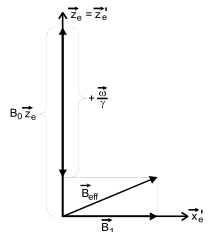
\includegraphics[width=0.3\textwidth]{bfeld.PNG}
  \caption{}
  \label{fig:bfeld}
\end{figure}
Für den Fall $B_0=\frac{\omega}{\gamma}$ entspricht grade $B_{eff}=B_1$
und die $\vec{M}$ dreht sich aus der $\vec{e}_z$-Achse heraus.
Der Drehwinkel $\delta(\Delta t)$ beträt dabei
\begin{align}
  \delta(\Delta t)=\gamma B_1 \Delta t.
\end{align}
Um die Magnetisierung um $\SI{90}{\degree}$ zu drehen beträgt die
Einstrahlungszeit
\begin{align}
  \Delta t_{90} = \frac{\pi}{2\gamma B_1}.
\end{align}
Die Magnetisierung zeigt somit in die $\vec{e}'_y$-Richtung, dies
entspricht einem $\SI{90}{\degree}$-Puls.
Für einen $\SI{180}{\degree}$-Puls beträgt dei Einstrahlungszeit
$\Delta t_{180}=2\Delta t_{90}$ und die Magnetisierung $\vec{M}$
zeigt in $-\vec{e}_z$-Richtung.
Durch Anwenden dieser diskreten Pulse lassen sich
wohldefinierte Nicht-Gleichgewichtszustände erzeugen.
Da die Magnetisierung nach den Pulsen wieder zu dem
Gleichgewichtszustand zurückstrebt, lassen sich so die
Relaxationszeiten $T_1$ und $T_2$ messen.

\subsection{Messmethoden}
\paragraph{Bestimmung der Relacationszeit $T_2$}
\begin{itemize}
  \item[-] Freier Induktionszerfall (FID)\\
  Für FID wird die Probe
  in ein homogenes Magnetfeld $B_0\vec{e}_z$ platziert.
  Zusätzlich befindet sich die Probe in einer
  Spule, die senkrecht zu dem Feld steht.
  Durch die Spule wird ein hochfequentes Magnetfeld
  mit der Frequenz $\omega_L=\gamma B_0$ eingestrahlt.
  Somit können wie in \ref{para:HF} $\SI{90}{\degree}$- oder $\SI{180}{\degree}$-Pulse
realisiert werden.
Bei dem freien Induktionszerfall wird die Probenmagnetisierung mit einem
$\SI{90}{\degree}$-Puls in $\vec{e}'_y$-Richtung rotiert. Nach abschalten des Pulses
führt die Magnetisierung dann eine Präzessionsbewegung in der
x-y-Ebene auf Grundes des noch bestehenden $B_0\vec{e}_z$ Feldes aus.
Die dadurch enstehende Induktionsspannung in der Spule wird in Abhängigkeit der Zeit aufgenommen.
Der Zerfall der transversalen Magnetisierung und somit auch abnehmen der
Induktionsspannung mit der Zeit, besitzt zwei Gründe.
Zum einen existiert kein perfektes homogens Magnetfeld bei einer
reale Apparatur und zum anderen
existieren Dipolfeldern der nächsten Nachbarn und Spins in der Elektronenhülle,
die ebenfalls eien Inhomogenität des Magnetfeldes in der Probe erzeugen.
Die Larmorfrequenzen der einzelnen Spins ist somit nicht mehr für alle Spins
gleich, sondern es existiert eine Verteilung der Larmorfrequenzen.
Dies führt zu einer Dephasierung
der Spins, da manche Spins schnell oder langsamer
als mit der Frequenz $\omega=\gamma B_0$ rotieren.
Die transversalen Magnetisierung nimmt deshalb mit der Zeit ab.
Messbar ist nur die Relaxationszeit $T_2^*$
mit
\begin{align}
  \frac{1}{T_2^*} = \frac{1}{T_2} + \frac{1}{T_{\Delta B}}
\end{align}
wobei $T_{\Delta B}$ der Zeitkonstante enspricht, die durch die Inhomogenität
des $B_0\vec{e}_z$ hervorgerufen wird.
Für ein hinreichend homogenens Feld ist $T_{\Delta B} \gg T_2$
und $T_2$ kann mit dem FID bestimmt werden.
Jedoch für $T_{\Delta B}$ \textless $T_2$ ist eine $T_2$-Bestimmung wegen
den apparativen Feldinhomogneitäten über FID nicht mehr möglich.

  \item[-] Spin-Echo-Verfahren\\
  Die Spin-Echo-Methode bietet eine Möglichkeit die apparativen Störeffekte
  bei der $T_2$-Bestimmung zu eliminieren.
  Dabei werden mit mindestens zwei HF-Pulsen benötigt.
  Mit einem $\SI{90}{\degree}$-Puls wird die Probenmagnetisierung in die
$\vec{e}'_y$-Richtung gedreht.
Wegen den verschiedenen Larmorfequenzen der einezelnen Spins, beginnt die Dephasierung.
Im rotierendem Koordinatensystem drehen somit Spins mit $\omega_{L_\text{Spin}}<\omega_{Hf}$
gegen und Spins mit $\omega_{L_\text{Spin}}>\omega_{Hf}$ mit dem
Uhrzeigersinn um die $\vec{e}_z$-Achse.
Bereits nach der Zeit $T_{\Delta B}$ ist die transversalen
Probenmagnetisierung durch
Auseinanderlaufen der Spins so gut wie verschwunden,
sodass kaum ein Induktionssignal
gemessen wird. Wird nach dem $\SI{90}{\degree}$-Puls
zu Zeitpunkt $\tau$
ein $\SI{180}{\degree}$-Puls
auf die Probe gegeben, wird nach $2\tau$, wie in Abbildung \ref{fig:hahn-echo} dargestellt, das sognannte Hahn-Echo beobachtet.
\begin{figure}
  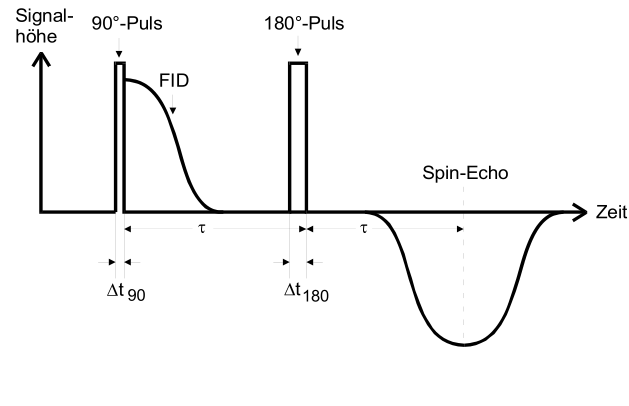
\includegraphics[width=0.8\textwidth]{hahn-echo.PNG}
  \caption{Hahn-Echo.}
  \label{fig:hahn-echo}
\end{figure}
Durch den $\SI{180}{\degree}$-Puls führen
die Spins eine Drehung um die
$\vec{e}'_x$-Achse aus und laufen wieder zusammen
zum Zeitpunkt $2\tau$ sind alle Spins wieder in Phase und eine
transversalen Probenmagnetisierung
erzeugt wieder ein Spingal in der Spule.
Der zeitliche Verlauf der Spins ist in Abbildung
\ref{fig:spin-echo} dargestellt.

\begin{figure}
  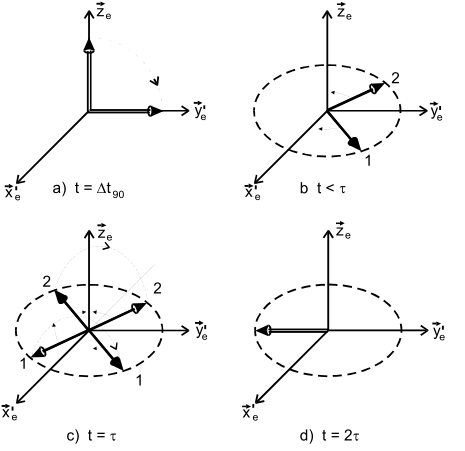
\includegraphics[width=0.8\textwidth]{spin-echo.PNG}
  \caption{Zeitlicher Verlauf des Hahn-Echos.}
  \label{fig:spin-echo}
\end{figure}

Das Hahn-Echo-Signal besitzt im vergleich zum Startsignal
ein anderes Vorzeichen, da die transversale
Magnetisierung zu Zeitpunkt $2\tau$ in $-\vec{e}_y$-Richtung zeigt.
Für $T_2\rightarrow\infty$ erreicht die betragsmäßige
Amplitude des Echos die
ursprüngliche Höhe vor dem FID.
Jedoch treten zu den reversiblen Dephasierungsprozessen auch
irreversible auf wie Wechselwirkung. Diese führen zur Abnahme der Echo-Stärke $M_Y$
,wie in Abbildung \ref{fig:tau_ver} dargestellt,
in Abhänigkeit von der Zeit in der Form
\begin{align}
  M_Y(t)=M_0 \exp\left(-\fra{t}{T_2}\right).
\end{align}

\begin{figure}
  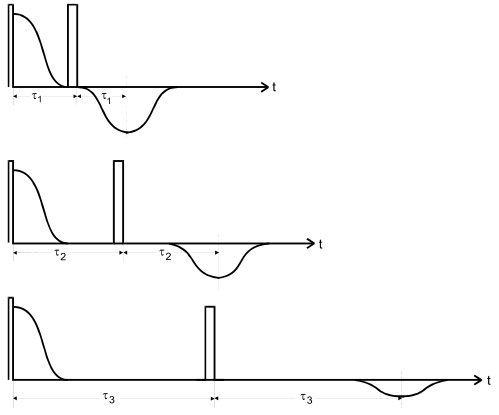
\includegraphics[width=0.8\textwidth]{tau_ver.PNG}
  \caption{Zeitlicher Verlauf des Hahn-Echos für unterschiedliche $\tau$.}
  \label{fig:tau_ver}
\end{figure}




  \item[-] Carr-Pucell- und Meilboom-Bill-Methode\\



\end{itemize}


% formeln
\begin{align}
% ddiffusionskonstante
M_Y(t) = M_0\exp\left(-\frac{t}{T_2}\right)
\symup{e}^(-\frac{D\gamma^2 G^2 t^3}{12} \label{}
\end{align}

\subsection{Messmethoden}
\paragraph{Spin-Echo-Methode}
\paragraph{Carr-Pucell-Methode}
\paragraph{Meiboom-Gill-Methode}
\subsection{Einfluss der Diffusion auf Relaxationsverfahren}


\cite{sample}
